\section{From SLR to MLR}


\begin{frame}{Recap: simple linear regression}
    The model with one regressor:
    \[
    y_i = \beta_0 + \beta_1 x_i + \varepsilon_i, \quad i=1,\dots,n.
    \]
    OLS estimators, written through the sample covariance, the variances and the correlation coefficient $r$:
    \begin{align}
        \hat\beta_1 &= \frac{S_{xy}}{S_{xx}} \label{eq:slr-b1}\\
        \hat\beta_0 &= \bar y - \hat\beta_1 \bar x, \notag\\
        \hat\sigma^2 &= \frac{\mathrm{SSE}}{n-2}. \label{eq:slr-s2}
    \end{align}
\end{frame}


\begin{frame}{Question: is one regressor enough?}
    Delivery time of a soft-drink route driver depends on the number of cases loaded ($x_1$) and the walking distance ($x_2$).

    Why not simply fit two separate SLRs, $y$ on $x_1$ and $y$ on $x_2$?

    \begin{itemize}
        \item The two regressors are typically correlated (more cases usually means longer distance).
        \item Each SLR slope then absorbs part of the effect of the omitted regressor, so it is not the effect of that regressor alone.
        \item Separate fits cannot answer ``what is the effect of one more case for a fixed distance?''.
        \item The residual variance is also larger because the omitted regressor's effect is left in the error.
    \end{itemize}
\end{frame}


\begin{frame}{Example: delivery time data}
    Montgomery, Peck \& Vining, Example 3.1 ($n=25$).
    \begin{itemize}
        \item $y$: delivery time (minutes)
        \item $x_1$: number of cases stocked
        \item $x_2$: distance walked by the driver (feet)
    \end{itemize}
    \begin{center}
        \small
        \begin{tabular}{cccc}
            \toprule
            Obs. & Time $y$ & Cases $x_1$ & Distance $x_2$ \\
            \midrule
            1  & 16.68 & 7 & 560 \\
            2  & 11.50 & 3 & 220 \\
            3  & 12.03 & 3 & 340 \\
            $\vdots$ & $\vdots$ & $\vdots$ & $\vdots$ \\
            25 & 10.75 & 4 & 150 \\
            \bottomrule
        \end{tabular}
    \end{center}
\end{frame}


\begin{frame}{From a line to a plane}
    \begin{columns}[T]
        \begin{column}{0.48\textwidth}
            \begin{itemize}
                \item SLR: a line in the $(x,y)$ plane.
                \item Two regressors: a plane in $(x_1,x_2,y)$ space.
                \item $k$ regressors: a hyperplane in $(k+1)$ dimensions.
                \item Residuals: vertical distances to the fitted surface.
            \end{itemize}
        \end{column}
        \begin{column}{0.48\textwidth}
            \begin{center}
                \resizebox{\linewidth}{!}{%
                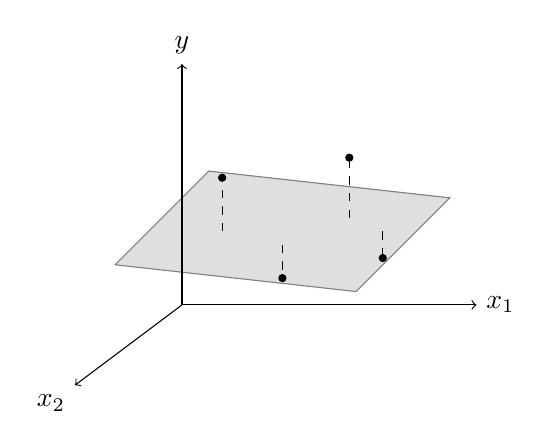
\begin{tikzpicture}[scale=0.85]
                    \fill[gray!25] (-1.0,0.6) -- (2.6,0.2) -- (4.0,1.6) -- (0.4,2.0) -- cycle;
                    \draw[gray] (-1.0,0.6) -- (2.6,0.2) -- (4.0,1.6) -- (0.4,2.0) -- cycle;
                    \draw[->] (0,0) -- (0,3.6) node[above] {$y$};
                    \draw[->] (0,0) -- (4.4,0) node[right] {$x_1$};
                    \draw[->] (0,0) -- (-1.6,-1.2) node[below left] {$x_2$};
                    \draw[dashed] (0.6,1.1) -- (0.6,1.9);
                    \draw[dashed] (1.5,0.9) -- (1.5,0.4);
                    \draw[dashed] (2.5,1.3) -- (2.5,2.2);
                    \draw[dashed] (3.0,1.1) -- (3.0,0.7);
                    \filldraw (0.6,1.9) circle (1.5pt);
                    \filldraw (1.5,0.4) circle (1.5pt);
                    \filldraw (2.5,2.2) circle (1.5pt);
                    \filldraw (3.0,0.7) circle (1.5pt);
                \end{tikzpicture}%
                }
            \end{center}
        \end{column}
    \end{columns}
\end{frame}


\section{The MLR model}


\begin{frame}{The MLR equation}
    With $k$ regressors and $n$ observations:
    \begin{align}
        y_i = \beta_0 + \beta_1 x_{i1} + \beta_2 x_{i2} + \cdots + \beta_k x_{ik} + \varepsilon_i, \quad i=1,\dots,n. \label{eq:mlr-scalar}
    \end{align}
    \begin{itemize}
        \item $x_{ij}$: value of regressor $j$ for observation $i$.
        \item $p = k+1$ unknown regression coefficients $\beta_0,\dots,\beta_k$ (including the intercept).
        \item $\varepsilon_i$: random error of observation $i$.
    \end{itemize}
\end{frame}


\begin{frame}{Meaning of the coefficients}
    \[
    \frac{\partial E[y\mid x_1,\dots,x_k]}{\partial x_j} = \beta_j, \quad j=1,\dots,k.
    \]
    \begin{itemize}
        \item $\beta_j$ is the change in the mean response per unit increase in $x_j$ \emph{when all other regressors are held fixed}.
        \item For this reason $\beta_1,\dots,\beta_k$ are called partial regression coefficients.
        \item $\beta_0$ is the mean response when all regressors are zero (meaningful only if that point is within the range of the data).
    \end{itemize}
\end{frame}


\begin{frame}{Question: interpreting the coefficients}
    In the delivery time model $y_i = \beta_0 + \beta_1 x_{i1} + \beta_2 x_{i2} + \varepsilon_i$, interpret $\beta_1$, $\beta_2$ and $\beta_0$ in words, with units.

    % Answer:
    % - beta_1: expected change in delivery time (minutes) for one additional case, for a fixed distance.
    % - beta_2: expected change in delivery time (minutes) for one additional foot of walking distance, for a fixed number of cases.
    % - beta_0: expected delivery time for zero cases and zero distance; an extrapolation with no practical meaning here.
\end{frame}


\begin{frame}{From $n$ equations to one matrix equation}
    Writing \eqref{eq:mlr-scalar} out for every observation:
    \begin{align*}
        y_1 &= \beta_0 + \beta_1 x_{11} + \cdots + \beta_k x_{1k} + \varepsilon_1 \\
        y_2 &= \beta_0 + \beta_1 x_{21} + \cdots + \beta_k x_{2k} + \varepsilon_2 \\
        &\;\;\vdots \\
        y_n &= \beta_0 + \beta_1 x_{n1} + \cdots + \beta_k x_{nk} + \varepsilon_n
    \end{align*}
    Stack the responses, the coefficients and the errors into vectors, and the regressor values into a matrix.
\end{frame}


\begin{frame}{The MLR model in matrix form}
    \begin{align}
        \mathbf y = \mathbf X\symbfit{\beta} + \symbfit{\varepsilon} \label{eq:mlr-matrix}
    \end{align}
    \[
    \underbrace{\mathbf y}_{n\times 1}, \qquad \underbrace{\mathbf X}_{n\times p}, \qquad \underbrace{\symbfit{\beta}}_{p\times 1}, \qquad \underbrace{\symbfit{\varepsilon}}_{n\times 1}.
    \]
\end{frame}


\begin{frame}{The vectors $\mathbf y$, $\symbfit{\beta}$, $\symbfit{\varepsilon}$}
    \[
    \mathbf y = \begin{pmatrix} y_1 \\ y_2 \\ \vdots \\ y_n \end{pmatrix}, \qquad
    \symbfit{\beta} = \begin{pmatrix} \beta_0 \\ \beta_1 \\ \vdots \\ \beta_k \end{pmatrix}, \qquad
    \symbfit{\varepsilon} = \begin{pmatrix} \varepsilon_1 \\ \varepsilon_2 \\ \vdots \\ \varepsilon_n \end{pmatrix}.
    \]
\end{frame}


\begin{frame}{The design matrix $\mathbf X$}
    \[
    \mathbf X = \begin{pmatrix}
        1 & x_{11} & x_{12} & \cdots & x_{1k} \\
        1 & x_{21} & x_{22} & \cdots & x_{2k} \\
        \vdots & \vdots & \vdots & & \vdots \\
        1 & x_{n1} & x_{n2} & \cdots & x_{nk}
    \end{pmatrix}
    \]
    \begin{itemize}
        \item Row $i$ is observation $i$; column $j$ is regressor $j$.
        \item The first column of ones corresponds to the intercept $\beta_0$.
    \end{itemize}
\end{frame}


\begin{frame}{Model assumptions}
    \begin{align}
        E[\symbfit{\varepsilon}] &= \mathbf 0, \label{eq:assump-mean}\\
        \mathrm{Var}(\symbfit{\varepsilon}) &= \sigma^2\mathbf I_n. \label{eq:assump-var}
    \end{align}
    \begin{itemize}
        \item $\mathbf X$ is fixed (non-random) and has full column rank, i.e.\ $\mathrm{rank}(\mathbf X)=p\le n$.
        \item No distributional assumption on $\symbfit{\varepsilon}$ is needed yet.
    \end{itemize}
\end{frame}


\begin{frame}{What does $\mathrm{Var}(\symbfit{\varepsilon})=\sigma^2\mathbf I_n$ say?}
    \[
    \mathrm{Var}(\symbfit{\varepsilon}) = E[\symbfit{\varepsilon}\symbfit{\varepsilon}'] =
    \begin{pmatrix}
        \sigma^2 & 0 & \cdots & 0 \\
        0 & \sigma^2 & \cdots & 0 \\
        \vdots & & \ddots & \vdots \\
        0 & 0 & \cdots & \sigma^2
    \end{pmatrix}
    \]
    \begin{itemize}
        \item Diagonal entries: every error has the same variance $\sigma^2$ (constant variance).
        \item Off-diagonal entries: errors of different observations are uncorrelated.
    \end{itemize}
\end{frame}


\begin{frame}{``Linear'' means linear in the parameters}
    Each of these is an MLR model:
    \begin{align*}
        y &= \beta_0 + \beta_1 x + \beta_2 x^2 + \varepsilon, \\
        y &= \beta_0 + \beta_1 x_1 + \beta_2 x_2 + \beta_{12} x_1 x_2 + \varepsilon.
    \end{align*}
    This one is not:
    \[
    y = \beta_0 e^{\beta_1 x} + \varepsilon.
    \]
    Polynomial and interaction terms are handled later in the course.
\end{frame}


\section{OLS estimation in matrix form}


\begin{frame}{The least-squares criterion}
    Choose $\symbfit{\beta}$ to minimise the sum of squared errors
    \begin{align}
        S(\symbfit{\beta}) = \sum_{i=1}^n \varepsilon_i^2 = \symbfit{\varepsilon}'\symbfit{\varepsilon} = (\mathbf y - \mathbf X\symbfit{\beta})'(\mathbf y - \mathbf X\symbfit{\beta}). \label{eq:ls-crit}
    \end{align}
\end{frame}


\begin{frame}{Expanding $S(\symbfit{\beta})$}
    \begin{align}
        S(\symbfit{\beta}) &= \mathbf y'\mathbf y - \symbfit{\beta}'\mathbf X'\mathbf y - \mathbf y'\mathbf X\symbfit{\beta} + \symbfit{\beta}'\mathbf X'\mathbf X\symbfit{\beta} \notag\\
        &= \mathbf y'\mathbf y - 2\symbfit{\beta}'\mathbf X'\mathbf y + \symbfit{\beta}'\mathbf X'\mathbf X\symbfit{\beta}. \label{eq:ls-expanded}
    \end{align}
    The second line combines the two middle terms.

    \svspace{1em}

    Why is $\mathbf y'\mathbf X\symbfit{\beta} = \symbfit{\beta}'\mathbf X'\mathbf y$?

    % Answer:
    % - y'X beta is a 1x1 matrix, i.e. a scalar.
    % - A scalar equals its own transpose: (y'X beta)' = beta'X'y.
\end{frame}


\begin{frame}{Two rules for differentiating with respect to a vector}
    For a constant vector $\mathbf a$ and a constant symmetric matrix $\mathbf A$:
    \[
    \frac{\partial\, \mathbf a'\symbfit{\beta}}{\partial\symbfit{\beta}} = \mathbf a,
    \qquad
    \frac{\partial\, \symbfit{\beta}'\mathbf A\symbfit{\beta}}{\partial\symbfit{\beta}} = 2\mathbf A\symbfit{\beta}.
    \]
    Apply with $\mathbf a=\mathbf X'\mathbf y$ and $\mathbf A=\mathbf X'\mathbf X$ (symmetric) to \eqref{eq:ls-expanded}.
\end{frame}


\begin{frame}{The normal equations}
    \begin{align}
        \frac{\partial S}{\partial\symbfit{\beta}} &= -2\mathbf X'\mathbf y + 2\mathbf X'\mathbf X\symbfit{\beta}, \notag\\
        \left.\frac{\partial S}{\partial\symbfit{\beta}}\right|_{\hat{\symbfit{\beta}}} &= \mathbf 0, \notag\\
        \mathbf X'\mathbf X\hat{\symbfit{\beta}} &= \mathbf X'\mathbf y. \label{eq:normal}
    \end{align}
    This is a system of $p$ linear equations in the $p$ unknowns $\hat\beta_0,\dots,\hat\beta_k$.
\end{frame}


\begin{frame}{The OLS estimator}
    If $\mathbf X'\mathbf X$ is invertible, the normal equations \eqref{eq:normal} have the unique solution
    \begin{align}
        \hat{\symbfit{\beta}} = (\mathbf X'\mathbf X)^{-1}\mathbf X'\mathbf y. \label{eq:ols}
    \end{align}
\end{frame}


\begin{frame}{When is $\mathbf X'\mathbf X$ invertible?}
    \begin{itemize}
        \item $\mathbf X'\mathbf X$ ($p\times p$) is invertible if and only if $\mathbf X$ has full column rank.
        \item That requires $n\ge p$ and no column of $\mathbf X$ being a linear combination of the other columns.
        \item If a regressor is (nearly) a linear combination of the others, $\mathbf X'\mathbf X$ is singular (nearly singular): this is the collinearity problem, treated in a later week.
    \end{itemize}
\end{frame}


\begin{frame}{Is $\hat{\symbfit{\beta}}$ a minimum?}
    \[
    \frac{\partial^2 S}{\partial\symbfit{\beta}\,\partial\symbfit{\beta}'} = 2\mathbf X'\mathbf X.
    \]
    \begin{itemize}
        \item For any $\mathbf a\neq\mathbf 0$: $\mathbf a'\mathbf X'\mathbf X\mathbf a = (\mathbf X\mathbf a)'(\mathbf X\mathbf a) = \|\mathbf X\mathbf a\|^2 > 0$, because full column rank gives $\mathbf X\mathbf a\neq\mathbf 0$.
        \item So $\mathbf X'\mathbf X$ is positive definite and $\hat{\symbfit{\beta}}$ is the unique minimiser of \eqref{eq:ls-crit}.
    \end{itemize}
\end{frame}


\begin{frame}[allowframebreaks]{SLR as a special Case of MLR}
    For SLR, $\mathbf X = [\mathbf 1\;\; \mathbf x]$ and
    \begin{align*}
        \mathbf X'\mathbf X &= \begin{pmatrix} n & \sum x_i \\ \sum x_i & \sum x_i^2 \end{pmatrix}, &
        \mathbf X'\mathbf y &= \begin{pmatrix} \sum y_i \\ \sum x_i y_i \end{pmatrix}.
    \end{align*}

    \framebreak

    Since $n\sum x_i^2 - (\sum x_i)^2 = nS_{xx}$,
    \[
    (\mathbf X'\mathbf X)^{-1} = \frac{1}{nS_{xx}}\begin{pmatrix} \sum x_i^2 & -\sum x_i \\ -\sum x_i & n \end{pmatrix}.
    \]
    The second entry of $(\mathbf X'\mathbf X)^{-1}\mathbf X'\mathbf y$ is
    \[
    \hat\beta_1 = \frac{n\sum x_i y_i - \sum x_i\sum y_i}{nS_{xx}} = \frac{nS_{xy}}{nS_{xx}} = \frac{S_{xy}}{S_{xx}},
    \]
    which is \eqref{eq:slr-b1}.
\end{frame}


\section{Fitted values, residuals and the hat matrix}


\begin{frame}{Fitted values and residuals}
    \begin{align}
        \hat{\symbfit{\beta}} &= (\mathbf X'\mathbf X)^{-1}\mathbf X' \mathbf y \notag\\ 
        \hat{\mathbf y} &= \mathbf X\hat{\symbfit{\beta}} = \mathbf X (\mathbf X'\mathbf X)^{-1}\mathbf X' \mathbf y = \mathbf H\mathbf y, \notag\\
        \mathbf H &= \mathbf X(\mathbf X'\mathbf X)^{-1}\mathbf X', \label{eq:H-def}\\
        \mathbf e &= \mathbf y - \hat{\mathbf y} = (\mathbf I-\mathbf H)\mathbf y. \label{eq:resid}
    \end{align}
    $\mathbf H$ is the $n\times n$ hat matrix: it puts the hat on $\mathbf y$.
\end{frame}


\begin{frame}{Properties of the hat matrix}
    \begin{align}
        \mathbf H' &= \mathbf H, \label{eq:H-sym}\\
        \mathbf H^2 &= \mathbf H, \label{eq:H-idem}\\
        \mathbf H\mathbf X &= \mathbf X. \label{eq:HX}
    \end{align}
    That is, $\mathbf H$ is symmetric and idempotent.
\end{frame}


\begin{frame}{Question: idempotency of $\mathbf H$}
    Prove \eqref{eq:H-idem} from the definition \eqref{eq:H-def}.

    % Answer:
    % H^2 = X(X'X)^{-1}X' X(X'X)^{-1}X' = X(X'X)^{-1}[X'X(X'X)^{-1}]X' = X(X'X)^{-1}X' = H.
\end{frame}


\begin{frame}{Properties of $\mathbf I-\mathbf H$}
    From \eqref{eq:H-sym}, \eqref{eq:H-idem} and \eqref{eq:HX}:
    \begin{align}
        (\mathbf I-\mathbf H)' &= \mathbf I-\mathbf H, \label{eq:IH-sym}\\
        (\mathbf I-\mathbf H)^2 &= \mathbf I-\mathbf H, \label{eq:IH-idem}\\
        (\mathbf I-\mathbf H)\mathbf X &= \mathbf 0. \label{eq:IHX}
    \end{align}
\end{frame}


\begin{frame}{Geometry of least squares}
    \begin{columns}[T]
        \begin{column}{0.48\textwidth}
            \begin{itemize}
                \item The columns of $\mathbf X$ span a $p$-dimensional subspace $\mathrm{col}(\mathbf X)$ of $\mathbb R^n$.
                \item $\hat{\mathbf y}=\mathbf H\mathbf y$ is the orthogonal projection of $\mathbf y$ onto $\mathrm{col}(\mathbf X)$.
                \item $\mathbf e$ is perpendicular to $\mathrm{col}(\mathbf X)$.
                \item $\hat{\mathbf y}$ is the point of $\mathrm{col}(\mathbf X)$ closest to $\mathbf y$, so $\hat{\symbfit{\beta}}$ minimises $\|\mathbf y-\mathbf X\symbfit{\beta}\|^2$.
            \end{itemize}
        \end{column}
        \begin{column}{0.48\textwidth}
            \begin{center}
                \resizebox{\linewidth}{!}{%
                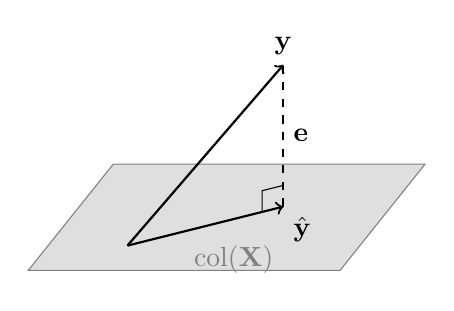
\begin{tikzpicture}[scale=0.9]
                    \fill[gray!25] (0,0) -- (4.4,0) -- (5.6,1.5) -- (1.2,1.5) -- cycle;
                    \draw[gray] (0,0) -- (4.4,0) -- (5.6,1.5) -- (1.2,1.5) -- cycle;
                    \node[gray] at (2.9,0.15) {$\mathrm{col}(\mathbf X)$};
                    \draw[->,thick] (1.4,0.35) -- (3.6,2.9) node[above] {$\mathbf y$};
                    \draw[->,thick] (1.4,0.35) -- (3.6,0.9) node[below right] {$\hat{\mathbf y}$};
                    \draw[dashed,thick] (3.6,0.9) -- (3.6,2.9) node[midway,right] {$\mathbf e$};
                    \draw (3.3,0.825) -- (3.3,1.125) -- (3.6,1.2);
                \end{tikzpicture}%
                }
            \end{center}
        \end{column}
    \end{columns}
\end{frame}


\begin{frame}{Orthogonality of residuals and regressors}
    \begin{align}
        \mathbf X'\mathbf e = \mathbf X'(\mathbf y-\mathbf X\hat{\symbfit{\beta}}) = \mathbf X'\mathbf y - \mathbf X'\mathbf X\hat{\symbfit{\beta}} = \mathbf 0, \label{eq:orth}
    \end{align}
    by the normal equations \eqref{eq:normal}. Consequences:
    \begin{itemize}
        \item First row of $\mathbf X'$ is a row of ones, so $\sum_i e_i = 0$.
        \item Row $j$ gives $\sum_i x_{ij}e_i = 0$ for each regressor.
        \item $\hat{\mathbf y}'\mathbf e = \hat{\symbfit{\beta}}'\mathbf X'\mathbf e = 0$.
    \end{itemize}
\end{frame}


\section{Delivery time example: OLS fit}


\begin{frame}{Computing $\mathbf X'\mathbf X$ and $\mathbf X'\mathbf y$}
    \begin{align*}
        \mathbf X'\mathbf X &= \begin{pmatrix} 25 & 219 & 10\,232 \\ 219 & 3\,055 & 133\,899 \\ 10\,232 & 133\,899 & 6\,725\,688 \end{pmatrix}, \\
        \mathbf X'\mathbf y &= \begin{pmatrix} 559.60 \\ 7\,375.44 \\ 337\,071.69 \end{pmatrix}.
    \end{align*}
\end{frame}


\begin{frame}{The inverse}
    \small
    \setlength{\arraycolsep}{4pt}
    \[
    (\mathbf X'\mathbf X)^{-1} =
    \begin{pmatrix}
        1.13\times10^{-1} & -4.45\times10^{-3} & -8.37\times10^{-5} \\
        -4.45\times10^{-3} & 2.74\times10^{-3} & -4.79\times10^{-5} \\
        -8.37\times10^{-5} & -4.79\times10^{-5} & 1.23\times10^{-6}
    \end{pmatrix}
    \]
\end{frame}


\begin{frame}{The fitted equation}
    \[
    \hat{\symbfit{\beta}} = (\mathbf X'\mathbf X)^{-1}\mathbf X'\mathbf y =
    \begin{pmatrix} 2.3412 \\ 1.6159 \\ 0.01438 \end{pmatrix}
    \]
    \[
    \hat y = 2.3412 + 1.6159\,x_1 + 0.01438\,x_2.
    \]
\end{frame}


\begin{frame}{Interpreting the fit}
    \begin{itemize}
        \item Each additional case adds about $1.62$ minutes to the delivery time, for a fixed distance.
        \item Each additional foot adds about $0.0144$ minutes (about $1.4$ minutes per $100$ ft), for a fixed number of cases.
        \item The SLR of $y$ on $x_1$ alone gives a slope of $2.18$, not $1.62$: cases and distance are correlated ($r=0.82$), and the SLR slope absorbs part of the distance effect.
    \end{itemize}
\end{frame}


\begin{frame}[fragile]{Verifying in R}
    \begin{verbatim}
y <- delivery$time
X <- cbind(1, delivery$cases, delivery$distance)

solve(t(X) %*% X, t(X) %*% y)

coef(lm(time ~ cases + distance,
        data = delivery))
\end{verbatim}
    \begin{itemize}
        \item \texttt{solve(A, b)} solves $\mathbf A\mathbf x=\mathbf b$ directly; it is numerically preferable to forming $\mathbf A^{-1}$ explicitly.
    \end{itemize}
\end{frame}


\section{Properties of the OLS estimators}


\begin{frame}{Linearity}
    \begin{align}
        \hat{\symbfit{\beta}} = \mathbf A\mathbf y, \qquad \mathbf A = (\mathbf X'\mathbf X)^{-1}\mathbf X'. \label{eq:linear}
    \end{align}
    $\mathbf A$ is a $p\times n$ matrix of constants (given $\mathbf X$), so every $\hat\beta_j$ is a linear combination of $y_1,\dots,y_n$.
\end{frame}


\begin{frame}{Decomposing $\hat{\symbfit{\beta}}$}
    Substitute the model \eqref{eq:mlr-matrix} into \eqref{eq:ols}:
    \begin{align}
        \hat{\symbfit{\beta}} &= (\mathbf X'\mathbf X)^{-1}\mathbf X'(\mathbf X\symbfit{\beta} + \symbfit{\varepsilon}) \notag\\
        &= \symbfit{\beta} + (\mathbf X'\mathbf X)^{-1}\mathbf X'\symbfit{\varepsilon}. \label{eq:decomp}
    \end{align}
    The estimator is the true $\symbfit{\beta}$ plus a linear function of the errors.
\end{frame}


\begin{frame}{Unbiasedness}
    Taking expectations in \eqref{eq:decomp} with $\mathbf X$ fixed, and using \eqref{eq:assump-mean}:
    \begin{align*}
        E[\hat{\symbfit{\beta}}] &= \symbfit{\beta} + (\mathbf X'\mathbf X)^{-1}\mathbf X'E[\symbfit{\varepsilon}] \\
        &= \symbfit{\beta}.
    \end{align*}
\end{frame}


\begin{frame}{The covariance matrix of a random vector}
    \[
    \mathrm{Var}(\hat{\symbfit{\beta}}) = E\big[(\hat{\symbfit{\beta}}-E[\hat{\symbfit{\beta}}])(\hat{\symbfit{\beta}}-E[\hat{\symbfit{\beta}}])'\big]
    \]
    is a $p\times p$ symmetric matrix:
    \begin{itemize}
        \item diagonal entries: $\mathrm{Var}(\hat\beta_j)$;
        \item off-diagonal entries: $\mathrm{Cov}(\hat\beta_i,\hat\beta_j)$.
    \end{itemize}
    For a constant matrix $\mathbf B$ and a random vector $\mathbf z$, directly from the definition,
    \begin{align}
        \mathrm{Var}(\mathbf B\mathbf z) = \mathbf B\,\mathrm{Var}(\mathbf z)\,\mathbf B'. \label{eq:var-rule}
    \end{align}
\end{frame}


\begin{frame}{Covariance matrix of $\hat{\symbfit{\beta}}$}
    \begin{align}
        \mathrm{Var}(\hat{\symbfit{\beta}}) &= \mathrm{Var}\big((\mathbf X'\mathbf X)^{-1}\mathbf X'\symbfit{\varepsilon}\big) \notag\\
        &= (\mathbf X'\mathbf X)^{-1}\mathbf X'\,\mathrm{Var}(\symbfit{\varepsilon})\,\mathbf X(\mathbf X'\mathbf X)^{-1} \notag\\
        &= \sigma^2(\mathbf X'\mathbf X)^{-1}\mathbf X'\mathbf X(\mathbf X'\mathbf X)^{-1} \notag\\
        &= \sigma^2(\mathbf X'\mathbf X)^{-1}. \label{eq:cov-beta}
    \end{align}
    The steps use \eqref{eq:decomp} (the constant $\symbfit{\beta}$ adds no variance), \eqref{eq:var-rule} and \eqref{eq:assump-var}.
\end{frame}


\begin{frame}{Reading the covariance matrix}
    Let $\mathbf C = (\mathbf X'\mathbf X)^{-1}$, with entries $C_{ij}$, $i,j=0,\dots,k$.
    \begin{align}
        \mathrm{Var}(\hat\beta_j) &= \sigma^2 C_{jj}, \label{eq:var-bj}\\
        \mathrm{Cov}(\hat\beta_i,\hat\beta_j) &= \sigma^2 C_{ij}, \quad i\neq j. \notag
    \end{align}
\end{frame}


\begin{frame}{Check: the SLR case}
    Using the inverse computed for SLR, with $\sum x_i^2 = S_{xx} + n\bar x^2$:
    \begin{align*}
        \mathrm{Var}(\hat\beta_1) &= \sigma^2\,\frac{n}{nS_{xx}} = \frac{\sigma^2}{S_{xx}}, \\
        \mathrm{Var}(\hat\beta_0) &= \sigma^2\,\frac{\sum x_i^2}{nS_{xx}} = \sigma^2\left(\frac1n + \frac{\bar x^2}{S_{xx}}\right), \\
        \mathrm{Cov}(\hat\beta_0,\hat\beta_1) &= -\sigma^2\,\frac{\sum x_i}{nS_{xx}} = -\sigma^2\,\frac{\bar x}{S_{xx}}.
    \end{align*}
    These are the familiar SLR results.
\end{frame}


\begin{frame}{Question: what makes $\mathrm{Var}(\hat\beta_j)$ large?}
    Using \eqref{eq:var-bj}, which features of the data and the design make the variance of $\hat\beta_j$ large?

    % Answer:
    % - Large error variance sigma^2.
    % - Small sample size n.
    % - Little spread in regressor x_j (as in SLR, Var(beta_1) = sigma^2 / S_xx).
    % - Strong linear relationship between x_j and the other regressors: C_jj becomes large. This is the collinearity problem.
\end{frame}


\section{The Gauss--Markov theorem}


\begin{frame}{Gauss--Markov theorem}
    Under \eqref{eq:assump-mean} and \eqref{eq:assump-var} (no normality needed), the OLS estimator $\hat{\symbfit{\beta}}$ is the best linear unbiased estimator (BLUE) of $\symbfit{\beta}$.
    \begin{itemize}
        \item Linear: a linear function of $\mathbf y$.
        \item Unbiased: $E[\hat{\symbfit{\beta}}]=\symbfit{\beta}$.
        \item Best: among all linear unbiased estimators, each $\hat\beta_j$, and more generally each $\mathbf c'\hat{\symbfit{\beta}}$, has the smallest variance.
    \end{itemize}
\end{frame}


\section{Distribution under normal errors}


\begin{frame}{Distribution of $\hat{\symbfit{\beta}}$}
    Add the assumption $\symbfit{\varepsilon}\sim N_n(\mathbf 0,\sigma^2\mathbf I_n)$. By \eqref{eq:decomp}, $\hat{\symbfit{\beta}}$ is a linear function of a normal vector, hence normal:
    \begin{align}
        \hat{\symbfit{\beta}} \sim N_p\big(\symbfit{\beta},\ \sigma^2(\mathbf X'\mathbf X)^{-1}\big). \label{eq:beta-dist}
    \end{align}
    The mean and covariance matrix are the ones derived above. This result drives the inference procedures in the coming weeks.
\end{frame}


\begin{frame}{Maximum likelihood under normal errors}
    The log-likelihood of $(\symbfit{\beta},\sigma^2)$ is
    \begin{align}
        \ell(\symbfit{\beta},\sigma^2) = -\frac n2\ln(2\pi\sigma^2) - \frac{1}{2\sigma^2}(\mathbf y-\mathbf X\symbfit{\beta})'(\mathbf y-\mathbf X\symbfit{\beta}). \label{eq:loglik}
    \end{align}
    For any fixed $\sigma^2$, maximising over $\symbfit{\beta}$ is the same as minimising $S(\symbfit{\beta})$ in \eqref{eq:ls-crit}, so the ML estimator of $\symbfit{\beta}$ equals the OLS estimator.
\end{frame}


\begin{frame}{Maximum likelihood estimator of $\sigma^2$}
    Setting $\partial\ell/\partial\sigma^2=0$ at $\symbfit{\beta}=\hat{\symbfit{\beta}}$ gives
    \begin{align}
        \hat\sigma^2_{\mathrm{ML}} = \frac{(\mathbf y-\mathbf X\hat{\symbfit{\beta}})'(\mathbf y-\mathbf X\hat{\symbfit{\beta}})}{n} = \frac{\mathrm{SSE}}{n}. \label{eq:mle-s2}
    \end{align}
    We show next that this estimator is biased.
\end{frame}


\section{Estimating the variance parameter \texorpdfstring{$\sigma^2$}{sigma squared}}


\begin{frame}{Residual sum of squares in matrix form}
    \begin{align}
        \mathrm{SSE} &= \mathbf e'\mathbf e = \mathbf y'(\mathbf I-\mathbf H)'(\mathbf I-\mathbf H)\mathbf y \notag\\
        &= \mathbf y'(\mathbf I-\mathbf H)\mathbf y. \label{eq:sse}
    \end{align}
    The first line uses \eqref{eq:resid}; the second uses \eqref{eq:IH-sym} and \eqref{eq:IH-idem}.
\end{frame}


\begin{frame}{Residuals as a function of the errors}
    \begin{align}
        \mathbf e &= (\mathbf I-\mathbf H)(\mathbf X\symbfit{\beta}+\symbfit{\varepsilon}) \notag\\
        &= (\mathbf I-\mathbf H)\symbfit{\varepsilon}, \label{eq:e-eps}\\
        \mathrm{SSE} &= \symbfit{\varepsilon}'(\mathbf I-\mathbf H)\symbfit{\varepsilon}. \label{eq:sse-eps}
    \end{align}
    The first line uses \eqref{eq:IHX}; \eqref{eq:sse-eps} follows as in \eqref{eq:sse}, now with \eqref{eq:e-eps}.
\end{frame}


\begin{frame}{Expectation of a quadratic form}
    For a constant symmetric matrix $\mathbf B$:
    \begin{align}
        E[\symbfit{\varepsilon}'\mathbf B\symbfit{\varepsilon}] &= E\big[\mathrm{tr}(\symbfit{\varepsilon}'\mathbf B\symbfit{\varepsilon})\big] = E\big[\mathrm{tr}(\mathbf B\symbfit{\varepsilon}\symbfit{\varepsilon}')\big] \notag\\
        &= \mathrm{tr}\big(\mathbf B\,E[\symbfit{\varepsilon}\symbfit{\varepsilon}']\big) = \sigma^2\,\mathrm{tr}(\mathbf B). \label{eq:quad-form}
    \end{align}
    \begin{itemize}
        \item A scalar equals its trace.
        \item $\mathrm{tr}(\mathbf M\mathbf N)=\mathrm{tr}(\mathbf N\mathbf M)$, and $E$ commutes with $\mathrm{tr}$.
        \item $E[\symbfit{\varepsilon}\symbfit{\varepsilon}']=\sigma^2\mathbf I_n$ by \eqref{eq:assump-mean} and \eqref{eq:assump-var}.
    \end{itemize}
\end{frame}


\begin{frame}{The trace of $\mathbf I-\mathbf H$}
    \begin{align}
        \mathrm{tr}(\mathbf H) &= \mathrm{tr}\big(\mathbf X(\mathbf X'\mathbf X)^{-1}\mathbf X'\big) = \mathrm{tr}\big((\mathbf X'\mathbf X)^{-1}\mathbf X'\mathbf X\big) \notag\\
        &= \mathrm{tr}(\mathbf I_p) = p, \notag\\
        \mathrm{tr}(\mathbf I_n-\mathbf H) &= n-p. \label{eq:tr-IH}
    \end{align}
\end{frame}


\begin{frame}{$E[\mathrm{SSE}]$ and an unbiased estimator of $\sigma^2$}
    Applying \eqref{eq:quad-form} with $\mathbf B=\mathbf I-\mathbf H$ to \eqref{eq:sse-eps}, and using \eqref{eq:tr-IH}:
    \begin{align}
        E[\mathrm{SSE}] &= \sigma^2(n-p), \label{eq:E-sse}\\
        \hat\sigma^2 &= \mathrm{MSE} = \frac{\mathrm{SSE}}{n-p}. \label{eq:mse}
    \end{align}
    $E[\mathrm{MSE}]=\sigma^2$. For $p=2$ this is the SLR estimator \eqref{eq:slr-s2}.
\end{frame}


\begin{frame}{Question: why divide by $n-p$?}
    The $n$ residuals are $e_i=y_i-\hat y_i$. Looking at \eqref{eq:E-sse}, why is the divisor of SSE $n-p$ and not $n$?
    What is the bias of $\hat\sigma^2_{\mathrm{ML}}$ in \eqref{eq:mle-s2}?

    % Answer:
    % - The residuals satisfy the p linear constraints X'e = 0 in (eq:orth), so only n-p of them are free: n-p degrees of freedom.
    % - E[SSE/n] = sigma^2 (n-p)/n < sigma^2, so the ML estimator underestimates sigma^2 (bias -p sigma^2 / n).
\end{frame}


\begin{frame}{Standard errors of the coefficients}
    Replace $\sigma^2$ by $\hat\sigma^2$ in \eqref{eq:cov-beta} and \eqref{eq:var-bj}:
    \begin{align}
        \widehat{\mathrm{Var}}(\hat{\symbfit{\beta}}) &= \hat\sigma^2(\mathbf X'\mathbf X)^{-1}, \notag\\
        \mathrm{se}(\hat\beta_j) &= \sqrt{\hat\sigma^2 C_{jj}}. \label{eq:se}
    \end{align}
\end{frame}


\begin{frame}{Delivery time data: $\hat\sigma^2$}
    \begin{itemize}
        \item $\mathrm{SSE} = 233.73$, with $n-p = 25-3 = 22$ degrees of freedom.
        \item $\hat\sigma^2 = \mathrm{MSE} = 233.73/22 = 10.62$.
        \item $\hat\sigma = 3.26$ minutes: the typical deviation of a delivery time from the fitted plane.
    \end{itemize}
\end{frame}


\begin{frame}{Delivery time data: standard errors}
    Using \eqref{eq:se}:
    \begin{center}
        \small
        \begin{tabular}{lcc}
            \toprule
            Coefficient & Estimate & Standard error \\
            \midrule
            $\beta_0$ (intercept) & 2.3412  & 1.0967 \\
            $\beta_1$ (cases)     & 1.6159  & 0.1707 \\
            $\beta_2$ (distance)  & 0.01438 & 0.003613 \\
            \bottomrule
        \end{tabular}
    \end{center}
\end{frame}


\section{Coefficient of determination and adjusted \texorpdfstring{$R^2$}{R squared}}


\begin{frame}{Sums of squares}
    \begin{align}
        \mathrm{SST} &= \sum_{i=1}^n (y_i-\bar y)^2 = \mathbf y'\mathbf y - n\bar y^2, \notag\\
        \mathrm{SSE} &= \mathbf y'\mathbf y - \hat{\symbfit{\beta}}'\mathbf X'\mathbf y, \notag\\
        \mathrm{SSR} &= \sum_{i=1}^n (\hat y_i-\bar y)^2 = \hat{\symbfit{\beta}}'\mathbf X'\mathbf y - n\bar y^2, \notag\\
        \mathrm{SST} &= \mathrm{SSR} + \mathrm{SSE}. \label{eq:ss-decomp}
    \end{align}
    The decomposition follows from the orthogonality \eqref{eq:orth}.
\end{frame}


\begin{frame}{The coefficient of determination}
    \begin{align}
        R^2 = \frac{\mathrm{SSR}}{\mathrm{SST}} = 1 - \frac{\mathrm{SSE}}{\mathrm{SST}}. \label{eq:r2}
    \end{align}
    \begin{itemize}
        \item The proportion of the variability in $y$ explained by the regressors; $0\le R^2\le 1$.
        \item Delivery time data: $R^2 = 0.9596$.
    \end{itemize}
\end{frame}


\begin{frame}{Question: adding a regressor}
    What happens to $R^2$ when a regressor is added to the model? Does it depend on whether the regressor is relevant?

    % Answer:
    % - R^2 never decreases, even for a regressor that is pure noise.
    % - Adding a column enlarges col(X), and the projection of y onto a larger subspace cannot be farther from y, so SSE cannot increase while SST is unchanged.
\end{frame}


\begin{frame}{Adding an irrelevant regressor}
    Add $z$, 25 independent $N(0,1)$ draws unrelated to the delivery time.
    \begin{center}
        \small
        \begin{tabular}{lccc}
            \toprule
            Model & $p$ & $R^2$ & MSE \\
            \midrule
            cases                       & 2 & 0.9305  & 17.484 \\
            cases, distance             & 3 & 0.9596  & 10.624 \\
            cases, distance, $z$        & 4 & 0.9597  & 11.109 \\
            \bottomrule
        \end{tabular}
    \end{center}
    $R^2$ increases slightly with the useless regressor, while the MSE goes up.
\end{frame}


\begin{frame}{Adjusted $R^2$}
    \begin{align}
        R^2_{\mathrm{adj}} &= 1 - \frac{\mathrm{SSE}/(n-p)}{\mathrm{SST}/(n-1)} = 1 - \frac{\mathrm{MSE}}{\mathrm{MST}}, \label{eq:adj-r2}\\
        &= 1 - \frac{n-1}{n-p}\,(1-R^2). \label{eq:adj-r2-alt}
    \end{align}
    $\mathrm{MST}=\mathrm{SST}/(n-1)$ is the sample variance of $y$.
\end{frame}


\begin{frame}{Why adjusted $R^2$ penalises useless regressors}
    \begin{itemize}
        \item $\mathrm{MST}$ does not depend on the model, so by \eqref{eq:adj-r2} $R^2_{\mathrm{adj}}$ increases if and only if $\mathrm{MSE}$ decreases.
        \item Adding a regressor lowers SSE but also lowers the degrees of freedom $n-p$ in \eqref{eq:mse}.
        \item The MSE decreases only if the drop in SSE outweighs the lost degree of freedom.
    \end{itemize}
\end{frame}


\begin{frame}{Adjusted $R^2$ in the example}
    \begin{center}
        \small
        \begin{tabular}{lccc}
            \toprule
            Model & $p$ & $R^2$ & $R^2_{\mathrm{adj}}$ \\
            \midrule
            cases                       & 2 & 0.9305  & 0.9275 \\
            cases, distance             & 3 & 0.9596  & 0.9559 \\
            cases, distance, $z$        & 4 & 0.9597  & 0.9539 \\
            \bottomrule
        \end{tabular}
    \end{center}
    $R^2_{\mathrm{adj}}$ rises when the relevant regressor (distance) is added and falls when the irrelevant $z$ is added.
\end{frame}


\begin{frame}{Properties of adjusted $R^2$}
    From \eqref{eq:adj-r2-alt}:
    \begin{itemize}
        \item For $p>1$, $R^2_{\mathrm{adj}} < R^2$ unless $R^2=1$.
        \item It can decrease when a regressor is added.
        \item It can be negative: $R^2_{\mathrm{adj}}<0$ whenever $R^2 < (p-1)/(n-1)$.
    \end{itemize}
\end{frame}


\begin{frame}{Caveats}
    \begin{itemize}
        \item A high $R^2$ or $R^2_{\mathrm{adj}}$ does not mean the model is adequate: the assumptions must be checked with residual analysis.
        \item $R^2_{\mathrm{adj}}$ is a descriptive measure, not a hypothesis test.
        \item Formal comparison of models is done later with F-tests and information criteria.
    \end{itemize}
\end{frame}


\section{Summary}


\begin{frame}{Summary}
    \begin{itemize}
        \item Model: $\mathbf y=\mathbf X\symbfit{\beta}+\symbfit{\varepsilon}$, with $E[\symbfit{\varepsilon}]=\mathbf 0$ and $\mathrm{Var}(\symbfit{\varepsilon})=\sigma^2\mathbf I_n$ \eqref{eq:mlr-matrix}.
        \item OLS: $\hat{\symbfit{\beta}}=(\mathbf X'\mathbf X)^{-1}\mathbf X'\mathbf y$ \eqref{eq:ols}; $\hat{\mathbf y}=\mathbf H\mathbf y$ is a projection onto $\mathrm{col}(\mathbf X)$.
        \item $\hat{\symbfit{\beta}}$ is unbiased with $\mathrm{Var}(\hat{\symbfit{\beta}})=\sigma^2(\mathbf X'\mathbf X)^{-1}$ \eqref{eq:cov-beta}, and is BLUE.
        \item $\hat\sigma^2=\mathrm{SSE}/(n-p)$ is unbiased for $\sigma^2$ \eqref{eq:mse}.
        \item $R^2$ never decreases when regressors are added; $R^2_{\mathrm{adj}}$ \eqref{eq:adj-r2} penalises the loss of degrees of freedom.
    \end{itemize}
\end{frame}


\begin{frame}{Next lecture}
    \begin{itemize}
        \item Inference on the regression coefficients: $t$-tests and confidence intervals.
        \item Test for significance of regression (F-test).
        \item Reading: Montgomery, Peck \& Vining, Chapter 3.
    \end{itemize}
\end{frame}


\appendix


\section{Proof of the Gauss--Markov Theorem}


\begin{frame}{Gauss--Markov: setup of the proof}
    Any linear estimator can be written
    \[
    \tilde{\symbfit{\beta}} = \big[(\mathbf X'\mathbf X)^{-1}\mathbf X' + \mathbf D\big]\mathbf y
    \]
    for some $p\times n$ matrix $\mathbf D$. Its expectation is $\symbfit{\beta} + \mathbf D\mathbf X\symbfit{\beta}$, so unbiasedness for every $\symbfit{\beta}$ requires
    \begin{align}
        \mathbf D\mathbf X = \mathbf 0. \label{eq:DX}
    \end{align}
\end{frame}


\begin{frame}{Gauss--Markov: the variance comparison}
    \begin{align*}
        \mathrm{Var}(\tilde{\symbfit{\beta}}) &= \sigma^2\big[(\mathbf X'\mathbf X)^{-1}\mathbf X' + \mathbf D\big]\big[\mathbf X(\mathbf X'\mathbf X)^{-1} + \mathbf D'\big] \\
        &= \sigma^2\big[(\mathbf X'\mathbf X)^{-1} + (\mathbf X'\mathbf X)^{-1}(\mathbf D\mathbf X)' \\
        &\qquad\quad + \mathbf D\mathbf X(\mathbf X'\mathbf X)^{-1} + \mathbf D\mathbf D'\big] \\
        &= \sigma^2(\mathbf X'\mathbf X)^{-1} + \sigma^2\mathbf D\mathbf D',
    \end{align*}
    where the last step uses \eqref{eq:DX}.
\end{frame}


\begin{frame}{Gauss--Markov: conclusion}
    \begin{itemize}
        \item $\mathbf a'\mathbf D\mathbf D'\mathbf a = \|\mathbf D'\mathbf a\|^2\ge 0$ for every $\mathbf a$, so $\mathbf D\mathbf D'$ is positive semidefinite.
        \item Hence $\mathrm{Var}(\tilde{\symbfit{\beta}}) - \mathrm{Var}(\hat{\symbfit{\beta}})$ is positive semidefinite, and $\mathrm{Var}(\mathbf c'\tilde{\symbfit{\beta}})\ge\mathrm{Var}(\mathbf c'\hat{\symbfit{\beta}})$ for every $\mathbf c$.
        \item Equality holds only for $\mathbf D=\mathbf 0$, i.e.\ $\tilde{\symbfit{\beta}}=\hat{\symbfit{\beta}}$.
    \end{itemize}
\end{frame}